%From https://egu2018.eu/PICO_how-to_guide_to_PICO.pdf
%Abstracted and templated by Brian Ballsun-Stanton, Macquarie University.
%original template by https://github.com/snowtechblog/pico-latex-presentation by Anselm Köhler

\documentclass[unknownkeysallowed,usepdftitle=false, parskip=full]{beamer}
% unknownkeysallowed is needed for mac and the newer latex version -> is more picky than before...
\usetheme[headheight=1cm,footheight=2cm]{boxes}
%\usetheme{default}


\usepackage{default}
\usepackage{graphicx}
%example pictures created via: http://lorempixel.com/1200/800/cats/Figure2/. Credit to http://lorempixel.com/images.php

\usepackage{epsfig}
\usepackage{siunitx}
\usepackage{color}
\usepackage{ifthen}
%usepackage{ragged2e}

\usepackage[T1]{fontenc}
\usepackage[utf8]{inputenc}
%https://tex.stackexchange.com/a/203804/5483

\usepackage[activate={true,nocompatibility},final,tracking=true,kerning=true,spacing=true,factor=1100,stretch=10,shrink=10]{microtype} % http://www.khirevich.com/latex/microtype/
\microtypecontext{spacing=nonfrench}

\usepackage{lipsum} % for dummy text only
\usepackage[UKenglish]{babel} %https://tex.stackexchange.com/a/27743 
\usepackage[pangram]{blindtext} % https://tex.stackexchange.com/a/48411

%\usepackage{parskip} % from https://tex.stackexchange.com/q/11622
%\setlength{\parskip}{12pt} 

%\setparsizes{\parindent}{12pt}{\parfillskip}

%\usepackage{etoolbox} % as per https://tex.stackexchange.com/a/24331
%\appto\chapterheadendvskip{\vspace{-1\parskip}}
%\setparsizes{\parindent}{50pt plus 20pt minus 30pt}{\parfillskip}

\setbeamertemplate{navigation symbols}{}%remove navigation symbols
\setbeamersize{text margin left=1cm,text margin right=1cm}

% some colors
\definecolor{grau}{gray}{.5}
\definecolor{slfcolor}{rgb}{1,0.5,0.1}
\definecolor{wslcolor}{rgb}{0.7,0.25,0}

% setup links
\hypersetup{%
	%linkbordercolor=green,%
	colorlinks=false,%
	pdfborderstyle={/S/U/W 0},%
	%pdfpagemode=FullScreen,%
	pdfstartpage=4%
	}

% setup some fonts
\setbeamerfont{title}{series=\bfseries, size=\small}
\setbeamerfont{author}{size*={5pt}{0pt}}
\setbeamerfont{institute}{size*={3pt}{0pt}}
\setbeamerfont{bodytext}{size=\scriptsize}
	
% Title setup	
\title{Improving Organisation of Music Production Projects}
\author{Dylan Wheeler, 42430704 (\texttt{dylan.wheeler@students.mq.edu.au})}
\institute{Macquarie University}
% add title in headbox
\setbeamertemplate{headline}
{\leavevmode
\begin{beamercolorbox}[width=1\paperwidth]{head title}
  % LOGO
  \begin{columns}[t, totalwidth=\textwidth]
  \begin{column}[c]{1.05cm}
     %
\includegraphics[width=1cm]{figure/logo1.png}
  \end{column}
  % TITLE
   \begin{column}[c]{10.6cm}
   \centering \usebeamerfont{title} \textcolor{slfcolor}{\inserttitle} \\
   \centering \usebeamerfont{author} \color[rgb]{0,0,0} \insertauthor \\
   \vspace{-0.05cm}
   \centering \usebeamerfont{institute} \insertinstitute
  \end{column}
  % PICTURE
  \begin{column}[c]{1.15cm}
    \hspace{0.005cm}
    %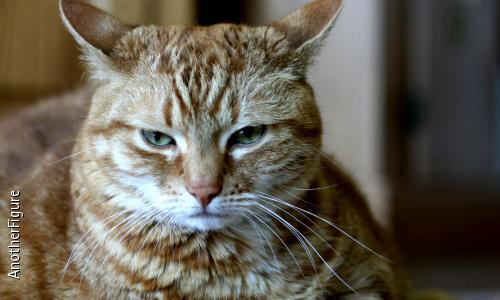
\includegraphics[width=1cm]{figure/figure1.png}
  \end{column}
  \end{columns}
  {\color{slfcolor}\hrule height 1pt\vspace{0.1cm}}
\end{beamercolorbox}%
}

% setup the navigation in footbox
% first set some button colors
\newcommand{\buttonactive}{\setbeamercolor{button}{bg=wslcolor,fg=white}}
\newcommand{\buttonpassive}{\setbeamercolor{button}{bg=slfcolor,fg=black}}
% now set up that the one active one gets the new color.
\newcommand{\secvariable}{nothing}
% therefore we write before each section (well, everything which should be part of the navi bar)
% the variable \secvariable to any name which is in the next function ...
\newcommand{\mysection}[1]{\renewcommand{\secvariable}{#1}
}
% ... compaired to strings in the following navibar definition ...
\newcommand{\tocbuttoncolor}[1]{%
 \ifthenelse{\equal{\secvariable}{#1}}{%
    \buttonactive}{%
    \buttonpassive}
 }
% ... here we start to set up the navibar. each entry is calling first the function \tocbuttoncolor with the argument which should be tested for beeing active. if active, then change color. afterwards the button is draw. so to change that, you need to change the argument in \toc..color, the first in \hyperlink and before each frames definition... A bit messed up, but works...
\newlength{\buttonspacingfootline}
\setlength{\buttonspacingfootline}{-0.2cm}
\setbeamertemplate{footline}
{\leavevmode
\begin{beamercolorbox}[width=1\paperwidth]{head title}
  {\color{slfcolor}\hrule height 1pt}
  \vspace{0.05cm}
  % set up the buttons in an mbox
  \centering \mbox{
    \tocbuttoncolor{abstract}
    \hyperlink{abstract}{\beamerbutton{2 Minute Madness}}
    
    \tocbuttoncolor{alternatives}
    \hspace{\buttonspacingfootline}
      \hyperlink{alternatives}{\beamerbutton{Alternatives}}

    \tocbuttoncolor{git}
    \hspace{\buttonspacingfootline}
      \hyperlink{git}{\beamerbutton{Git}}
      

    \hspace{\buttonspacingfootline}
    \tocbuttoncolor{scripts}
      \hyperlink{scripts}{\beamerbutton{Scripts}}
%    \tocbuttoncolor{slab}
%    \hspace{\buttonspacingfootline}
%      \hyperlink{slab}{\beamerbutton{Section 4}}
%    \tocbuttoncolor{minor}
%    \hspace{\buttonspacingfootline}
%      \hyperlink{minor}{\beamerbutton{Section 5}}
    \tocbuttoncolor{credits}
    \hspace{\buttonspacingfootline}
      \hyperlink{credits}{\beamerbutton{Credits}}
    % this last one should normaly not be used... it will open the preferences to change the 
    % behaviour of the acrobat reader in fullscreen -> usefull in pico...
    \setbeamercolor{button}{bg=white,fg=black}
    % for presentation
    %\hspace{-0.1cm}\Acrobatmenu{FullScreenPrefs}{\beamerbutton{\#}}
    % for upload
    
     
\Acrobatmenu{FullScreenPrefs}{\vspace{0.3cm}\hspace{0.24cm}\mbox{%
      
\includegraphics[height=0.04\textheight,keepaspectratio]{%
	  figure/CreativeCommons_Attribution_License.eps}%
	  }}
   }
    \vspace{0.05cm}
\end{beamercolorbox}%
}


\begin{document}


%%%%%%%%%%%%%%%%%%%%%%%%%%%%%%%%%%%%%%%%%%%%%%%%%%%%%%%%%%%%%%%%%%%%%%%%%%
\mysection{abstract}
%%%%%%%%%%%%%%%%%%%%%%%%%%%%%%%%%%%%%%%%%%%%%%%%%%%%%%%%%%%%%%%%%%%%%%%%%%
\begin{frame}\label{\secvariable}

\usebeamerfont{bodytext}




%Original template: https://github.com/snowtechblog/pico-latex-presentation by Anselm Köhler

\begin{columns}
    \begin{column}{0.4\textwidth}
    \parbox{\linewidth}{
    \textbf{The Problem:}

    \vspace{12pt}

    Keeping music production projects
    
    organised is hard because:
    \begin{itemize}
        \item Need to have many versions of the same thing.
        \item Metaprojects are a thing.
        \item Need documentation, especially in research contexts.
        \item Need to work quickly and intuitively.
    \end{itemize}
    }
    \end{column}

    \begin{column}{0.5\textwidth}
    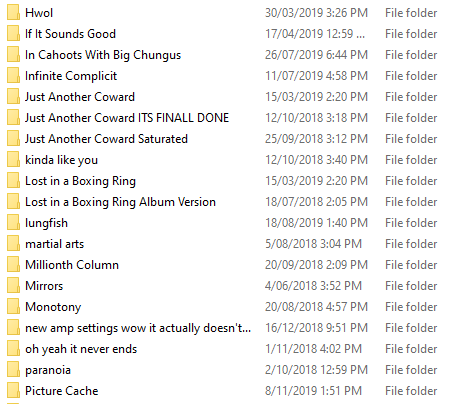
\includegraphics[width=1\textwidth,height=0.45\textheight,keepaspectratio]{figure/clutter-folder.png}
    \vspace{4pt}
    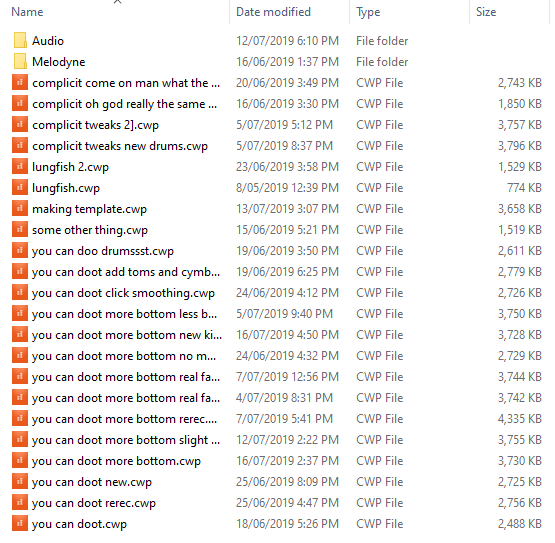
\includegraphics[width=1\textwidth,height=0.45\textheight,keepaspectratio]{figure/clutter-project.png}
    \end{column}
\end{columns}

   
\end{frame}

\begin{frame}\label{\secvariable}
\parbox{\linewidth}{
\textbf{The Solution:}
\begin{itemize}
    \item Take some time to actually think about project organisation.
    \item Use version control. In this case Git. Solutions built specifically for music production were found to be unsuitable. Git actually works very well with just a couple of caveats.
    \item Write some custom scripts to handle some aspects of project creation and management. These work with Git.
    \item Actually use the tools.
\end{itemize}
}
\end{frame}

%%%%%%%%%%%%%%%%%%%%%%%%%%%%%%%%%%%%%%%%%%%%%%%%%%%%%%%%%%%%%%%%%%%%%%%%%%
\mysection{alternatives}
%%%%%%%%%%%%%%%%%%%%%%%%%%%%%%%%%%%%%%%%%%%%%%%%%%%%%%%%%%%%%%%%%%%%%%%%%%
\begin{frame}\label{\secvariable}
\parbox{\linewidth}{
\textbf{Existing Alternatives Were Unsuitable}
\vspace{12pt}
\begin{itemize}
    \item Built in DAW "version control" tools earn their scare quotes. Not reliable.
    \vspace{12pt}
    \item There are a couple of online platforms for managing music production projects, including version control BUT:
    \begin{enumerate}
        \item They only support some DAWs, this solution will work with any.
        \item I don't trust them.
    \end{enumerate}
\end{itemize}
}
\end{frame}

%%%%%%%%%%%%%%%%%%%%%%%%%%%%%%%%%%%%%%%%%%%%%%%%%%%%%%%%%%%%%%%%%%%%%%%%%%
\mysection{git}
%%%%%%%%%%%%%%%%%%%%%%%%%%%%%%%%%%%%%%%%%%%%%%%%%%%%%%%%%%%%%%%%%%%%%%%%%%
\begin{frame}\label{\secvariable}
\parbox{\linewidth}{
    \textbf{Overall Git works well to version control music production projects, BUT:}
    \begin{itemize}
        \item The actual audio files are large and USUALLY don't change after creation. Tell Git to ignore them.
        \item On rare occasions producers might destructively edit audio files. Git cannot help you in this case (assuming you've ignored the audio files).
        \item The project files have proprietary formats. You can't do the kind of useful version comparisons you might be able to do with code or text files. A tool that COULD compare (e.g.) EQ settings between different versions of a project would be enormously useful, but obviously well beyond the scope of this unit to develop.
        \item If you're using a DAW that allows you to save your project as one big file that includes both the project settings and audio data, don't do that.
    \end{itemize}
}  
\end{frame}

%%%%%%%%%%%%%%%%%%%%%%%%%%%%%%%%%%%%%%%%%%%%%%%%%%%%%%%%%%%%%%%%%%%%%%%%%%
\mysection{scripts}
%%%%%%%%%%%%%%%%%%%%%%%%%%%%%%%%%%%%%%%%%%%%%%%%%%%%%%%%%%%%%%%%%%%%%%%%%%
\begin{frame}\label{\secvariable}
\parbox{\linewidth}{
\textbf{Custom scripts take care of the following things:}
\begin{itemize}
    \item Creating new projects in the repository with unique names and all documentation present (users can set up their own project templates).
    \item Creating metaprojects with same conditions.
    \item Associating/disassociating projects with metaprojects.
    \item Switching projects from being active to being archived.
\end{itemize}
}
\end{frame}

%%%%%%%%%%%%%%%%%%%%%%%%%%%%%%%%%%%%%%%%%%%%%%%%%%%%%%%%%%%%%%%%%%%%%%%%%%
\mysection{credits}
%%%%%%%%%%%%%%%%%%%%%%%%%%%%%%%%%%%%%%%%%%%%%%%%%%%%%%%%%%%%%%%%%%%%%%%%%%
\begin{frame}\label{\secvariable}
  
Source for this presentation is available at: https://github.com/MQ-FOAR705/Wheeler.Presentation

\vspace{12pt}

Original template: https://github.com/snowtechblog/pico-latex-presentation by Anselm Köhler
  
\end{frame}



\end{document}
